\documentclass[10pt]{beamer}
%\usepackage{amsmath}
\usepackage{url}
\mode<presentation>
{
    \usetheme{Warsaw}
    % \usetheme{default}

        \setbeamercovered{transparent}
}

\newcommand{\ls}[1]
{\dimen0=\fontdimen6\the\font
    \lineskip=#1\dimen0
        \advance\lineskip.5\fontdimen5\the\font
        \advance\lineskip-\dimen0
        \lineskiplimit=.9\lineskip
        \baselineskip=\lineskip
        \advance\baselineskip\dimen0
        \normallineskip\lineskip
        \normallineskiplimit\lineskiplimit
        \normalbaselineskip\baselineskip
        \ignorespaces
}

\title{Hands on Intro - Git}
\author{Amjith Ramanujam}
\institute{twitter: amjith\_\\
blog: amjith.blogspot.com}

\date{}
\begin{document}
\begin{frame}
    \titlepage
\end{frame}

\begin{frame}
    \frametitle{Getting Started}
    Download \url{http://amjith.com/tmp/cab.tar.gz}
    \begin{block}{Getting Started}
        \begin{itemize}
            \item git init \\
            \item git add .\\
            \item git commit -m ``Initial Commit.''
        \end{itemize}
    \end{block}
\end{frame}

\begin{frame}
    \frametitle{Configuration}
    \begin{block}{User Name}
        \begin{itemize}
            \item git config --global user.name "Amjith Ramanujam"   \\
            \item git config --global user.email "amjith.r@gmail.com"\\
        \end{itemize}
    \end{block}
    \pause
    \begin{block}{gitignore}
        \begin{itemize}
            \item .gitignore\\
            \item git config --global core.excludefiles /home/amjith/.gitignore\\
        \end{itemize}
    \end{block}
    \textasciitilde/.gitconfig
    \pause
    \begin{block}{Git Cloning}
        \begin{itemize}
		\item git clone git://github.com/amjith/Cows\_and\_Bulls-Game.git
        \end{itemize}
    \end{block}
\end{frame}

\begin{frame}
    \frametitle{Basic Operations}
    \begin{block}{Staging}
        \begin{itemize}
            \item git commit -m ``Modification to the success and fail messages.''
        \end{itemize}
    \end{block}
    \begin{center}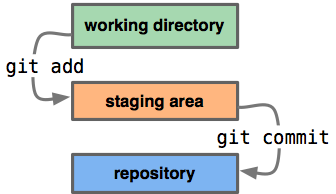
\includegraphics{images/index1.png}\end{center}
        \begin{block}{Interactive Staging}
            \begin{itemize}
                \item Useful for code review.
                \item Partial checkins. 
            \end{itemize}
        \end{block}
\end{frame}

\begin{frame}
    \frametitle{Basic Operations}
    \begin{itemize}
        \item git log
        \item git status
        \item git diff [--cached]
        \item git show
        \item git checkout
        \item git revert
    \end{itemize}
    \begin{block}{aliases}
        \begin{itemize}
            \item git config --global alias.ci commit
            \item git config --global alias.co checkout
            \item git config --global alias.st status
            \item git config --global alias.br branch
        \end{itemize}
    \end{block}
\end{frame}

\begin{frame}
    \frametitle{SVN Comparison}
    \begin{block}{Git vs SVN}
        \begin{table}[h]
            %\caption{Git Vs SVN}
            \centering
            \begin{tabular}{|c|c|}
                \hline
                & \\ [-1ex]
                git init & svnadmin create repo \\[.25ex]
                \hline
                git clone & svn checkout \\[.25ex]
                \hline
                git checkout & svn switch \\[.25ex]
                \hline
                git commit  & svn commit \\[.25ex]
                \hline
                git pull  & svn update \\[.25ex]
                \hline
                git push  & svn commit \\[.25ex]
                \hline
                git log  & svn log \\[.25ex]
                \hline
            \end{tabular}
        \end{table}
    \end{block}
\end{frame}

\begin{frame}
    \frametitle{Distributed Version Control}
    \begin{block}{Advantages}
        \begin{itemize}
            \item Local Branches - create/checkout/merge
            \item Patch/Apply - send/apply patches
            \item Central Repos - add origin - github
            \item Sharing Repos - ssh between friends
        \end{itemize}
    \end{block}
\end{frame}

\begin{frame}
    \frametitle{Advanced Topics}
    \begin{block}{}
        \begin{itemize}
            \item git stash
            \item git rebase
        \end{itemize}
    \end{block}
\end{frame}

\begin{frame}
    \frametitle{References}
    \begin{block}{References}
        \begin{itemize}
            \item Git Tips: \url{http://www.gitready.com}
            \item Successful Git branching: \url{http://nvie.com/posts/a-successful-git-branching-model/}
            \item Public Repo: \url{http://www.kernel.org/pub/software/scm/git/docs/user-manual.html\#setting-up-a-public-repository}
            \item Git hosting: \url{http://github.com}
        \end{itemize}
    \end{block}
\end{frame}
\end{document}
